\begin{framed}

Objetivos:
\begin{itemize}
    \item Repasar la descripción de fluidos mediante ecuaciones diferenciales.
    \item Repasar las leyes de conservación.
\end{itemize}

Contenidos:
\begin{itemize}
    \item Introducción y generalidades.
    \item Repaso: cinemática de una partícula de fluido.
    \item Repaso: Ecuaciones diferenciales de conservación. 
    \begin{itemize}
        \item Masa: Continuidad.
        \item Momentum: Navier-Stokes.
        \item Energía.
    \end{itemize}
\end{itemize}

Bibliografía:
\begin{itemize}
    \item White, F. M. (2008) Mecánica de Fluidos. McGraw-Hill. Sexta edición. Secciones 4.1-4.4
    \item Fox, R. W., Pritchard, P. J. y McDonald, A. T. (2009) Introduction to Fluid Mechanics. John Wiley \& Sons. Secciones 5.1-5.4
\end{itemize}
\end{framed}

En esta primera clase estudiaremos el análisis diferencial del movimiento de un fluido. 
Para esto, iniciaremos viendo como se describe el movimiento de un elemento diferencial de fluido, para luego aplicar las leyes de conservación de masa, cantidad de movimiento, y energía sobre el elemento diferencial.
 Este material fue visto en el curso Mecánica de Fluidos General, sin embargo, lo repasamos para estar en la misma página con respecto a lo que viene hacia adelante.

\section*{Elemento diferencial en movimiento}
Digamos que tenemos un flujo y que somos capaces de hacer un pequeño cuadrado con tinta al tiempo $t=0$.
Este pequeño cuadrado servirá como nuestro elemento diferencial a analizar.
Digamos que esperamos una pequeña cantidad de tiempo $\delta t$ y le sacamos una foto \mbox{?`}Qué ocurrió con el cuadrado que dibujamos? Algo como lo que muestra la Figura \ref{fig:elemento_diferencial}
%
\begin{figure}[h!]
\centering
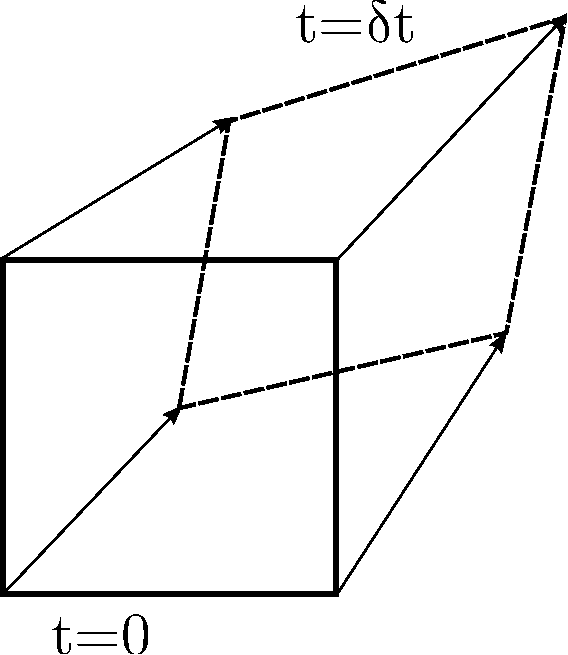
\includegraphics[width=0.4\textwidth]{clase01/elemento_diferencial.pdf}
\caption{Deformación y traslación de un elemento diferencial tras un tiempo $\delta t$}
\label{fig:elemento_diferencial}
\end{figure}

La razón por la que el elemento de fluido de la Figura \ref{fig:elemento_diferencial} se deformó es que la velocidad no es constante dentro del mismo. 
En la figura, las flechas representan el cambio de posición de las esquinas en el tiempo $\delta t$. 
Al ser la misma cantidad de tiempo $\delta t$ en los cuatro casos, las flechas nos entregan una idea de la velocidad en esos puntos, la cual es distinta en cada caso.
De hecho, si $\delta t=1$s, las flechas serían exactamente la velocidad. 

De esta forma, podemos concluir que existe un campo de velocidad $\mathbf{V}(\mathbf{x},t) = (u(\mathbf{x},t),v(\mathbf{x},t),w(\mathbf{x},t))$, donde $\mathbf{x}=(x,y,z)$, que puede ir variando en el espacio y tiempo.

\subsubsection*{Campo de velocidades}
Nuestro modelo se basa en considerar el fluido como un continuo. 
Por lo tanto, en vez de tener velocidades discretas de cada molécula de agua, analizamos el comportamiento promedio, y podemos representar la velocidad como una función continua:
%
\begin{equation}
\mathbf{V}(\mathbf{x},t) = u(\mathbf{x},t)\ihat+v(\mathbf{x},t)\jhat+w(\mathbf{x},t)\khat,
\end{equation}
%
donde, como antes, $\mathbf{x} = (x,y,z)$. 

Se habrán dado cuenta que la partícula de fluido se mueve con el fluido, por lo tanto, $\mathbf{x}=\mathbf{x}(t)$. 
Estudiemos la aceleración de la partícula.
Si el elemento de fluido estuviese detenido, simplemente $\mathbf{a}=\frac{\partial \mathbf{V}}{\partial t}$ nos entregaría la aceleración, sin embargo, al estar moviéndose con el fluido, utilizaremos la notación $\frac{D}{Dt}$, que se conoce como derivada material o total:
%
\begin{equation}\label{eq:acel}
\mathbf{a} = \frac{D\mathbf{V}}{Dt} = \frac{Du}{Dt}\ihat+\frac{Dv}{Dt}\jhat+\frac{Dw}{Dt}\khat.
\end{equation}
%
Veamos lo que ocurre en el eje $x$. 
Por regla de la cadena, queda:
%
\begin{equation}
\frac{Du}{Dt} = \frac{\partial u}{\partial x}\frac{Dx}{Dt} +\frac{\partial u}{\partial y}\frac{Dy}{Dt} +\frac{\partial u}{\partial z}\frac{Dz}{Dt}+ \frac{\partial u}{\partial t}\frac{Dt}{Dt}
\end{equation}
%
pero,
\begin{align}
\frac{Dx}{Dt} &= u \nonumber\\
\frac{Dy}{Dt} &= v \nonumber\\
\frac{Dz}{Dt} &= w 
\end{align}
%
y llegamos a
%
\begin{equation}
\frac{Du}{Dt} = u\frac{\partial u}{\partial x} + v\frac{\partial u}{\partial y} + w\frac{\partial u}{\partial z} + \frac{\partial u}{\partial t}
\end{equation}
%
En 3 dimensiones, esto es
%
\begin{equation}
\mathbf{a} = \frac{D\mathbf{V}}{Dt} = \frac{\partial \mathbf{V}}{\partial t} + u\frac{\partial \mathbf{V}}{\partial x} + v\frac{\partial \mathbf{V}}{\partial y} + w\frac{\partial \mathbf{V}}{\partial z} = \underbrace{\frac{\partial \mathbf{V}}{\partial t}}_\text{local} + \underbrace{(\mathbf{V}\cdot\nabla)\mathbf{V}}_\text{convectiva},
\end{equation}
%
donde el primer término se conoce como aceleración local, y el segundo como aceleración convectiva.
Noten que un elemento de fluido se puede estar acelerando incluso en una situación estacionaria (donde $\partial \mathbf{V}/\partial t=0$).

\subsubsection*{Movimiento de un elemento diferencial}
La Figura \ref{fig:elemento_diferencial} muestra como un elemento de fluido cuadrado se mueve y deforma. 
Uno puede imaginar que mientras más complicado el campo de velocidad, se hace más difícil de entender la deformación.
Para facilitar el análisis, la Figura \ref{fig:deformacion} describe el movimiento y deformación en cuatro partes: traslación, deformación lineal, rotación y deformación angular.
%
\begin{figure}[h!]
\centering
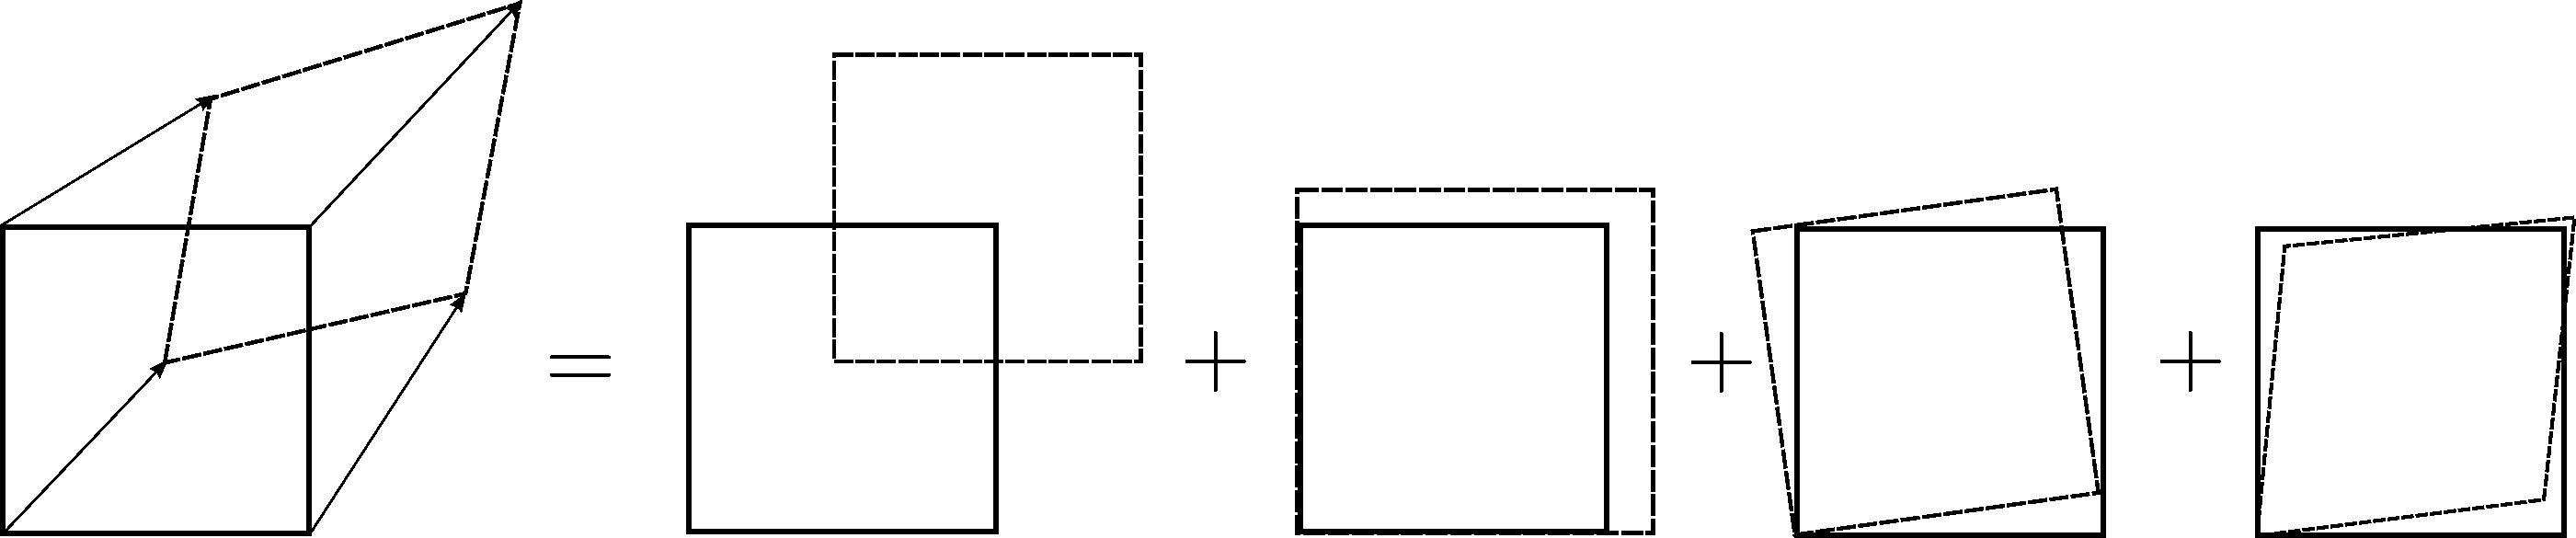
\includegraphics[width=\textwidth]{clase01/deformacion.pdf}
\caption{Traslación, deformación lineal, rotación y deformación angular de un elemento de fluido}
\label{fig:deformacion}
\end{figure}
%
Analicemos cada una de estas.

\paragraph{Traslación y deformación lineal.}
La traslación como aparece en el primer término de la Figura \ref{fig:deformacion} ocurre cuando la velocidad del fluido es constante dentro del volúmen.
Ese es un caso muy simple \mbox{?`}Qué ocurre cuando no es así? Probemos con el caso unidimensional de la Figura \ref{fig:deformacion_lineal}:
%
\begin{figure}[h!]
\centering
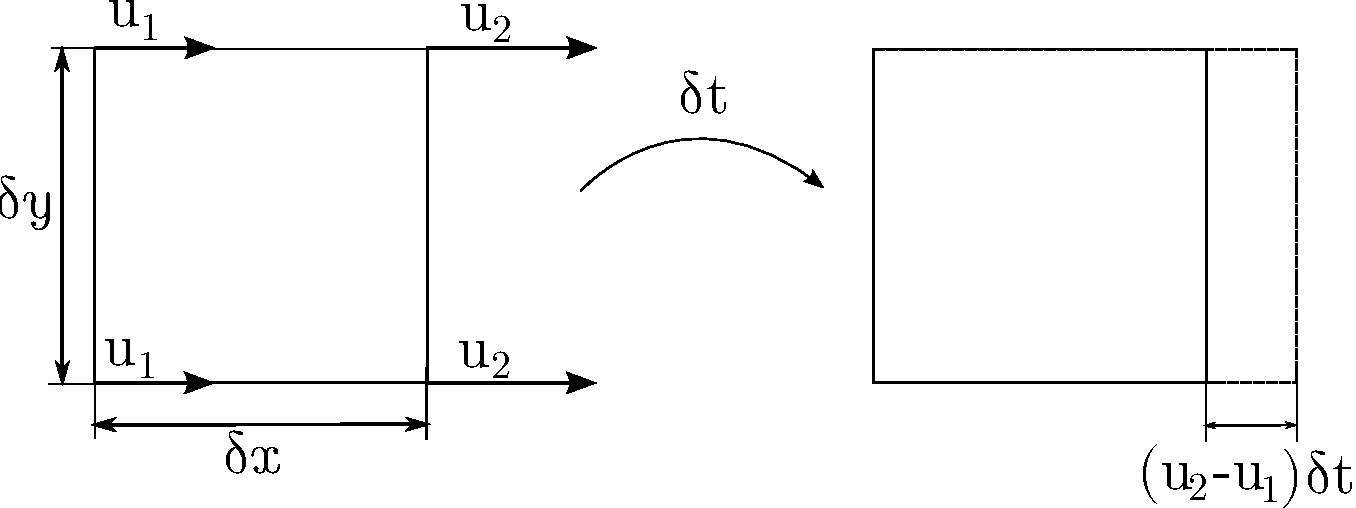
\includegraphics[width=0.7\textwidth]{clase01/deformacion_lineal.pdf}
\caption{Deformación lineal en el eje x.}
\label{fig:deformacion_lineal}
\end{figure}


